\documentclass[spanish, fleqn]{article}
\usepackage{babel}
\usepackage{fourier}
\usepackage{amsmath, amsfonts, amsthm, fourier}
\usepackage{float}

\usepackage{graphicx}

\usepackage[colorlinks, urlcolor=blue]{hyperref}

\usepackage{mathtools}
\DeclarePairedDelimiter{\ceil}{\lceil}{\rceil}
\DeclarePairedDelimiter{\floor}{\lfloor}{\rfloor}

\setlength{\parindent}{0pt}

\title{Ayudantía 3 - Algoritmos y Complejidad\\
Algoritmos Voraces}
\author{Exponential Complexers}
\date{}

\begin{document}
\maketitle

\thispagestyle{empty}
\section{Introducción}
% PLACEHOLDER
Para demostrar que un algoritmo voraz es óptimo, tenemos que demostrar las siguientes tres propiedades:
\begin{itemize}
\item \textbf{Elección voraz}: Que si elegimos $\hat{p}$, existe alguna solución óptima $\Pi^*$ que incluya $\hat{p}$.
\\ Podemos demostrar por reducción al absurdo , suponiendo que de todas las soluciones óptimas ninguna incluye $\hat{p}$ y mostrar, por ejemplo, que se podría obtener una solución mejor agregando $\hat{p}$ contradiciendo la optimalidad de las originales. 
\\ A veces es posible demostrar que todas las soluciones óptimas deben contener a $\hat{p}$, en este caso se estaría demostrando más de lo necesario, pero aun es suficiente.
\item \textbf{Estructura inductiva}: Que al momento de recortar el problema $P$, resultando en un problema $P'$ una solución de dicho problema $P'$, llamémosla $\Pi'^*$ unida a $\{\hat{p}\}$ siempre forman una solución factible para $P$, llamémosla $\Pi$.
\\ Lo que importa es elegir $P'$ correctamente, no siempre basta con elegir $P'=P-\{\hat{p}\}$ a veces hay que eliminar más cosas de manera que no queden \emph{objetos} que sean afectados de alguna manera por la elección de $\hat{p}$, osea, que $P'$ esté libre de condiciones externas.
\begin{figure}[H]
\centering
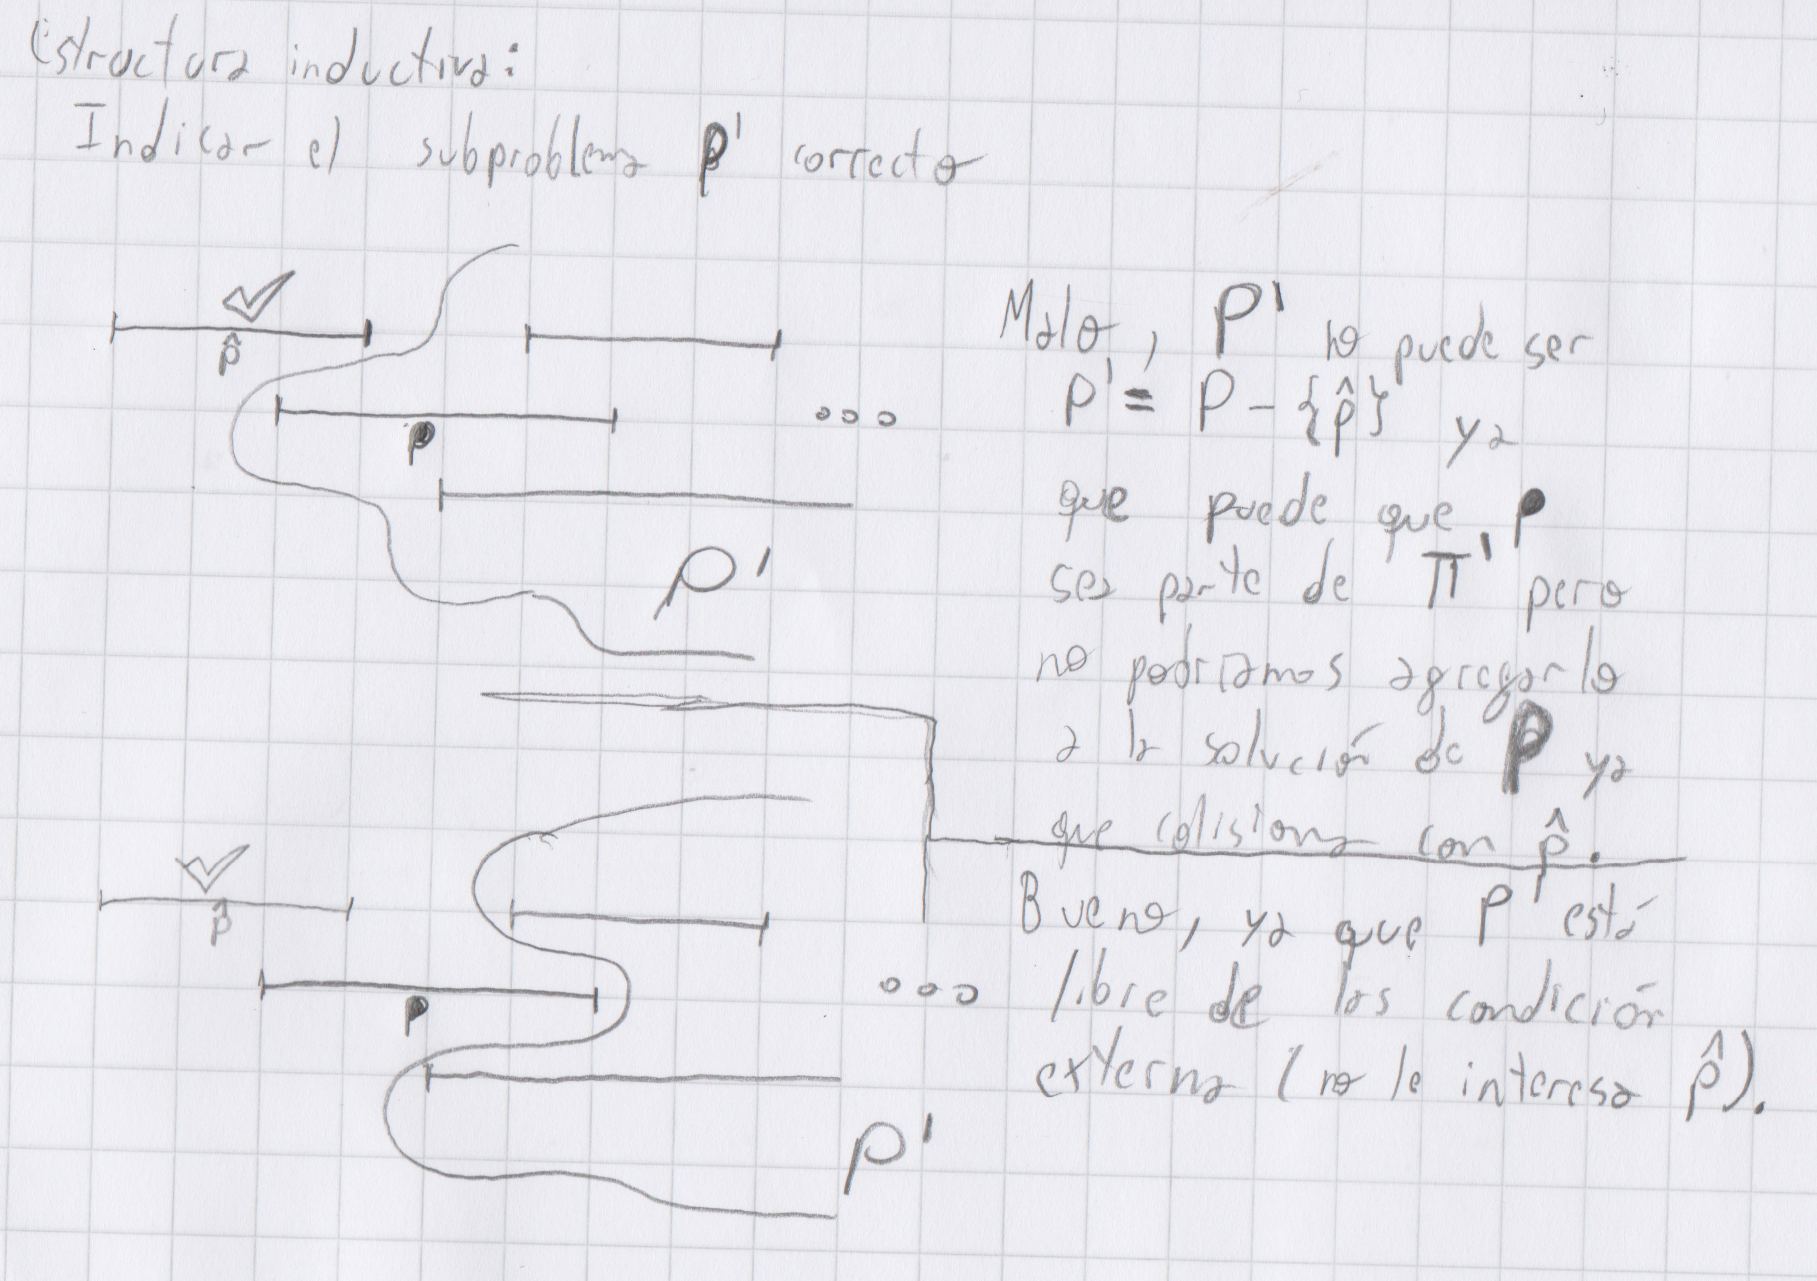
\includegraphics[scale=0.6]{imagen}
\caption{Definir correctamente el problema $P'$.}
\end{figure}

\item \textbf{Sub-estructura óptima}: Debemos demostrar ahora, que la solución $\Pi= \{\hat{p}\} \cup {\Pi'}^*$ para el problema $P$ (siendo ${\Pi'}^*$ la solución óptima para el problema $P'$), es óptima.
\\ Generalmente podremos demostrar por reducción al absurdo, suponiendo que existe una solución mejor. Si se trata de un problema donde ``mejor'' está definido por la cardinalidad de la solución, habría que demostrar que no es posible una solución con menos (o más) de $|{\Pi'}^*|+1$ elementos para el problema $P$.
\\ Nada nos impide apoyarnos en lo demostrado en \emph{elección voraz} para lograr nuestro cometido.
\end{itemize}

\section{Ejercicios}

\begin{enumerate}

\item Se tiene dos conjuntos de valores reales positivos $\langle a_1, a_2,...,a_n\rangle$ y $\langle b_1, b_2,...,b_n\rangle$, tal que:
\begin{align*}
a_1 \geq a_2 \geq ... \geq a_n &\quad \text{y}
\\ b_1 \geq b_2 \geq ... \geq b_n
\end{align*}
Se busca maximizar:
\begin{align*}
\sum_{i=1}^n a_{i} b_{\phi(i)}
\end{align*}
Donde $\phi: [1..n] \rightarrow [1..n]$ es una biyección. Dicho de otra forma, se busca hacer un matching entre $a$'s y $b$'s que maximice la suma de las multiplicaciones entre los pares.

Demostrar que el algoritmo voraz de emparejar $a_1$ y $b_1$ (osea, los más grandes de cada conjunto) en cada paso es óptimo.

\paragraph{Solución}
\begin{itemize}
\item \textbf{Elección voraz}: Cualquier solución óptima $\Pi^*$ que no tenga $a_1b_1$, tendrá que tener $a_ib_1$ y $a_1b_j$, en dicha solución podemos hacer un swap, intercambiando $a_ib_1$ y $a_1b_j$ por $a_1b_1$ y $a_ib_j$, en dicho caso la diferencia en la sumatoria será:
\begin{align*}
a_1b_1 + a_ib_j - a_ib_1 - a_1b_j
\end{align*}
Este valor es positivo ya que:
\begin{align*}
(a_1 - a_i) \geq 0 \wedge (b_1 - b_j) \geq 0
\\\Rightarrow (a_1 - a_i)(b_1 - b_j) &\geq 0 \\\Rightarrow a_1b_1 + a_ib_j - a_ib_1 - a_1b_j &\geq 0
\end{align*}
Por lo tanto, o la solución $\Pi^*$ que no incluye $a_1b_1$ y es óptima no existe (en caso de que la expresión siempre sea positiva) o existe una solución óptima que incluye $a_1b_1$.
\item \textbf{Sub-estructura inductiva}: Tras hacer el match $a_1b_1$ sacamos $a_1$ y $b_1$ del problema, quedando un problema $P'$ en que a cualquier solución $\Pi'$ (si vemos las soluciones como conjuntos de pares) se le puede agregar $a_1b_1$ para formar una solución factible de $P$.
\item \textbf{Sub-estructura óptima}: De elección voraz se obtuvo que existe una solución óptima que incluye $a_1b_1$ para $P$ y la mejor forma posible de elegir los otros pares sería la solución óptima a $P'$ dada por $\Pi'^*$, como el criterio de optimalidad es al suma de los pares, la única forma de maximizar esta suma es maximizando los sumandos y por lo tanto, $\Pi = \{a_1b_1\} \cup \Pi'^*$ debe óptima para $P$. \\ (No existe la posibilidad de que una solución a $P'$ diferente aumente más $a_1b_1 + \sum_{i=2}^n a_{i} b_{\phi(i)}$, pues dicha solución no puede aumentar otra cosa que $\sum_{i=2}^n a_{i} b_{\phi'(i)}$ y si pudiera hacerlo $\Pi'^*$ ya no sería óptima)z.
\end{itemize}

\item Suponga que se tiene un conjunto de números ordenados representados en un árbol binario, proponga un algoritmo voraz eficiente, que encuentre el número más cercano a un número $n$ dentro del árbol.

\begin{figure}[H]
\centering
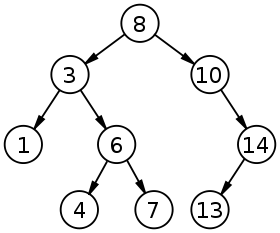
\includegraphics[scale=0.5]{arbol}
\caption{Árbol binario con número ordenados, el camino para el número más cercano a $9$ sería $\{8,10,14,13\}$.}
\end{figure}

Demuestre su optimalidad.

\paragraph{Solución} Nuestro algoritmo consistiría en bajar por el árbol de la misma manera que lo haríamos buscando dicho número, de manera que si el el número $n$ que buscamos es mayor que el nodo actual, buscamos hacia la derecha y si es menor buscamos hacia la izquierda, si estamos en un nodo que tiene el valor buscado, dejamos de buscar, pues no habrá un número más cerca que el mismo número.

Ahora, no necesariamente el nodo al que lleguemos estará más cerca de $n$, pero al menos uno de los nodos más cercanos a $n$ de todo árbol estará en dicho camino --esto porque nuestra elección, como ya veremos, siempre va por el lado que tendrá uno de estos nodos (si es que no hemos pasado por él ya)--.

Por lo anterior, no podemos hablar de una solución como un sólo nodo (si lo viéramos así tampoco podríamos hacer estructura inductiva), debemos pensar en la solución como un camino en el árbol; donde consideramos un camino como óptimo si incluye uno de los nodos más cercanos a $n$ en el árbol.

Consideraremos que un problema involucra un árbol, y $\hat{p}$ se puede elegir de una de sus dos ramas, sólo en el problema original (que involucra el árbol completo) agregamos el nodo raíz a la solución (en los otros no será necesario hacerlo ya que lo abremos agregado como $\hat{p}$ en el paso anterior).

Demostramos las 3 propiedades:
\begin{enumerate}
\item \textbf{Elección voraz}: Si se avanza por el nodo $\hat{p}$, desde el nodo padre $p$, existe una solución óptima $\Pi^*$ que incluye $\hat{p}$.
\\ Si $n=p$ se termina el problema, no hay que agregar nada a la solución. 
\\ Caso contrario, sea $k$ el número en el árbol que está más cerca de $n$:
\begin{itemize}
\item Si $n<p$: se elige como $\hat{p}$ el nodo hijo menor de $p$.\\ Como $k$ es más cercano a $n$ que $p$, $k<p$; por lo tanto, para llegar a $k$ se debe pasar por $\hat{p}$, a menos que ya se haya hecho, pero en ese caso la solución ya sería óptima.
\item Si $n>p$: se elige como $\hat{p}$ el nodo hijo mayor de $p$.\\ Como $k$ es más cercano a $n$ que $p$, $k>p$; por lo tanto, para llegar a $k$ se debe pasar por $\hat{p}$, a menos que ya se haya hecho, pero en ese caso la solución ya sería óptima.
\end{itemize}
\item \textbf{Estructura inductiva}: Si se elige pasar por $\hat{p}$, la solución será $(\hat{p})$ más la solución al problema con el sub-árbol que proyecta $\hat{p}$. Notar que eliminamos todo el resto del árbol.
\item \textbf{Sub-estructura óptima}: Demostramos que no existe una solución mejor que la que encontraremos yendo por $\hat{p}$ (osea resolviendo el sub-problema del sub-árbol que proyecta $\hat{p}$).
\\ Otra vez los dos casos:
\begin{itemize}
\item Si $\hat{p}<p$: se eligió $\hat{p}$ porque $n<p$.
\\ En el otro árbol solo tendremos números mayores que $p$, por lo tanto nunca estarán más cerca de $n$ que el mismo $p$ y no hay solución mejor fuera de la óptima del subproblema.
\item Si $\hat{p}>p$: se eligió $\hat{p}$ porque $n>p$.
\\ En el otro árbol solo tendremos números menores que $p$, por lo tanto nunca estarán más cerca de $n$ que el mismo $p$ y no hay solución mejor fuera de la óptima del subproblema.
\end{itemize}

\end{enumerate}

\item Describa un algoritmo voraz para representar un número $n$ con el menor número de monedas de los valores $20$,$10$,$5$ y $1$. Demuestre que es óptimo.

\paragraph{Solución} El algoritmo consiste en agregar la moneda $k$ de mayor valoración tal que $k\leq n$, luego se sigue, resolviendo el problema para $n-k$. Cuando llegamos $n$ sea igual a alguna moneda, agregamos dicha moneda y terminamos.

Demostramos las 3 propiedades:
\begin{enumerate}
\item \textbf{Elección voraz}: Supongamos que existe una solución $\Pi_n^*$ óptima que no elige la moneda de mayor valor $m$ (tal que $m\leq n$), entonces, poseé un subconjunto de monedas que suman $m$ (por los tipos de monedas que hay), si reemplazamos ese subconjunto por la moneda $m$, tendríamos una solución mejor, pero $\Pi_n^*$ era óptima, contradicción.
\item \textbf{Estructura inductiva}: Tras elegir la moneda $m$, resulta el subproblema $P_{n-m}$ de representar $n-m$ con monedas, El conjunto de monedas $\Pi_{n-m} \cup \{m\}$, es solución factible para $P_n$ ya que suman $m$ y no hay restricciones externas al resolver $P_{n-m}$ (la moneda elegida no afecta para nada cómo resolveremos $P_{n-m}$).
\item \textbf{Sub-estructura óptima}: Debemos demostrar que $\Pi_n= \Pi_{n-m}^* \cup \{m\}$, es óptima, osea, no se puede resolver el problema $P_n$ con menos monedas que $|\Pi_{n-m}^*|+1$.
\\ Supongamos lo contrario, entonces es posible reemplazar un subconjunto de monedas de $\Pi_{n-m}^*$ por otro subconjunto de menos o igual cantidad de monedas de manera que la suma de estas monedas aumente en $m$.
\\Si hacemos este cambio queda una solución para $P_n$ con $|\Pi_{n-m}^*|$ monedas, por lo visto en (a), existe una solución igual de óptima que tiene una moneda $m$, si sacamos esa moneda, tendríamos una solución para $P_{n-k}$ que requeriría $|\Pi_{n-m}^*|-1$ monedas y por lo tanto $\Pi_{n-m}^*$ no sería óptima; contradicción.
\end{enumerate}

\item Describa un algoritmo voraz para representar un número $n$ con el menor número de monedas de los valores $5$,$3$,$2$ y $1$. Demuestre que es óptimo.
\\\textbf{Advertencia: Este ejercicio es experimental y feo}, no garantizo que su tiempo sea retribuído.
%\\\textbf{Tip 1} Bastan $\ceil*{\frac{n}{5}}+1$ monedas para representar cualquier número $n$.
%\\\textbf{Tip 2} Nunca se requieren menos de $\ceil*{\frac{n}{5}}$ monedas para representar cualquier número $n$.
\paragraph{Solución} El algoritmo, como siempre, consiste en agregar la moneda $k$ de mayor valoración tal que $k\leq n$, luego se sigue, resolviendo el problema para $n-k$.

%Primero notamos una propiedad muy interesante, podemos escribir:
%\begin{align*}
%n &= 5\cdot x + y \qquad, x \in \mathbb{N}, y \in \{ 0,1,2,3,4 \} 
%\end{align*}

%Para simplificar, remitámonos a pensar que las soluciones sólo pueden tomar monedas en orden decreciente (reducir el problema), esto tiene sentido ya que al final buscamos un \textbf{conjunto} de monedas (no importa el orden).

%Además, notemos que si no se tuvieran monedas de $5$, el óptimo necesariamente será con tantas monedas de $3$ como fuera posible, más una moneda de $1$ o $2$.

Primero notamos que no hay forma de lograr ningún número $n>5$ sin utilizar monedas de $5$ que sea más óptima:
\\ Lo mejor que se puede tener sin usar monedas de $5$ es $\ceil*{\frac{n}{3}}$.
\\ Por otro lado, usando tantas monedas de $5$ como se pueda se obtendría $\ceil*{\frac{n}{5}}+1$ monedas, ya que si $n= 5i+4$, nos queda $4$ sobrando, tendremos que usar $2$ monedas más.

¿Cuándo $\ceil*{\frac{n}{3}}$ es mejor que $\ceil*{\frac{n}{5}}+1$?
\\ Si $n>7$ ya claramente no puede ser mejor. Por lo tanto sólo queda $n=6$, y en ese caso, sólo se igualan.

Demostramos las 3 propiedades:
\begin{enumerate}
\item \textbf{Elección voraz}: Supongamos que la solución óptima mejor $\Pi_n^*$ que no incluye la moneda de mayor denominación posible $m$ (a diferencia de nuestra solución $\Pi_n$) y en su lugar agrega una moneda $k$.
\begin{itemize}
\item Si $m=5$, por lo demostrado anteriormente, no es posible hacer una solución mejor con monedas de menor valor.
\item Si $m<5$, por lo demostrado anteriormente, $n<5$ y en ese caso, siempre podremos usar la moneda de mayor valor disponible para formar una solución óptima ($1$,$2$,$3$ se pueden hacer sólo con esta moneda, y $4$ siempre se puede formar con $3$ y $1$, no pudiendo hacerlo con menos monedas).
\end{itemize}
%Puesto que $k$ sólo puede ser $3$,$2$ o $1$, el número mínimo de monedas sería $|\Pi_n^*|=\ceil*{\frac{n}{k}}$. Y si esto fuera cierto:
%\begin{align*}
%|\Pi_n^*| = & &
%\\ & \ceil*{\frac{n}{k}} \geq 1+\ceil*{\frac{n-m}{k}} \geq 1+|\Pi_{n-m}^*| &
%\\ & & = |\Pi_n|
%\end{align*}
%Por lo tanto, $|\Pi_n^*|$ no podría ser mejor que $|\Pi_n|$.
\item \textbf{Estructura inductiva}: Una vez elegida la moneda $m$, a partir de la solución óptima del problema $P_{n-m}$, llámese $\Pi_{n-m}$ se puede agregar la moneda $m$ para crear una solución viable para el problema $\Pi_{n}$.
\item \textbf{Subestructura óptima}: Tenemos que demostrar que teniendo el óptimo $|\Pi_{n-m}^*|$, no existe ninguna forma de obtener $|\Pi_n|$ en que no tengamos que agregar al menos una moneda (pues entonces $|\Pi_n|$ no sería óptimo).
\\ Notemos que las monedas que no son monedas de $5$ para alguna solución óptima de $P_{n-m}$ sólo pueden ser $\{1\},\{2\},\{3\},\{2,2\},\{3,1\}$ y también podemos agregar $\{3,3\}$ como caso especial, en que pueden reemplazar un grupo de $\{5,1\}$ si fuera necesaria una moneda de $1$; estos conjuntos de monedas serían lo único que podríamos cambiar para lograr formar una solución óptima de $P_{n}$ (ya que las otras monedas, de $5$, necesariamente tendrán que ser parte de la solución de $P_{n}$).
\\Veamos los casos para $m$:
\begin{itemize}
\item Si $m=5$, no tenemos manera de reemplazar estos conjuntos de monedas de manera que su valor aumente en $5$ y no aumente el número de monedas.
\item Si $m=3$ Tampoco podremos hacerlo, ya que en el conjunto de reemplazo no podremos poner monedas de $5$ pues $n<5$.
\item Si $m=2$ Tampoco podremos hacerlo, ya que en el conjunto de reemplazo no podremos poner monedas de $3$ pues $n<3$, a lo más podríamos llevar la moneda de $1$ a valer $2$.
\item Si $m=1$ necesariamente $n=1$, y por lo tanto estamos en el caso en que tenemos $0$ monedas, necesariamente habrá que agregar $1$.
\end{itemize}
%\item \textbf{Subestructura óptima}: Vemos que $\Pi_{n}$ sólo requiere  una moneda más que $\Pi_{n-m}^*$, por lo tanto, $\Pi_{n}$ sería óptima siempre y cuando no exista una manera de representar $n$ sin aumentar el número de monedas de $\Pi_{n-m}^*$.
%\\ Por nuestra simplificación, sabemos que $\Pi_{n-m}^*$ no poseé monedas mayores que $m$; entonces existen dos posibilidades:
%\begin{itemize}
%\item Si $m=5$ claramente agregar esta moneda adicional será necesario.
%\item Si $m<5$, $\Pi_{n-m}^*$ necesariamente consistirá en $\floor*{\frac{n-m}{k}}$ monedas $k$ y, opcionalmente, una moneda de menor valor.
%\\ Promover la moneda de menor valor no serviría ya que necesitaríamos hacerlo en $m$ unidades, y quedaríamos con una moneda mayor que $m$. Por lo tanto hay que agregar $1$ moneda al menos.
%\end{itemize}

\end{enumerate}
\end{enumerate}
\end{document}
